
\begin{frame}[ctb!]
\frametitle{LLNL Model Thermal Diffusivity Sensitivity}
\footnotesize{
By varying the thermal diffusivity of the disposal system from $0.1-3\times 
10^{-6} [m^2\cdot s^{-1}]$, this sensitivity analysis succeeds in capturing the domain of 
thermal diffusivities witnessed in high thermal diffusivity salt deposits as 
well as low thermal diffusivity clays.

\begin{figure}[htbp!]
\begin{center}
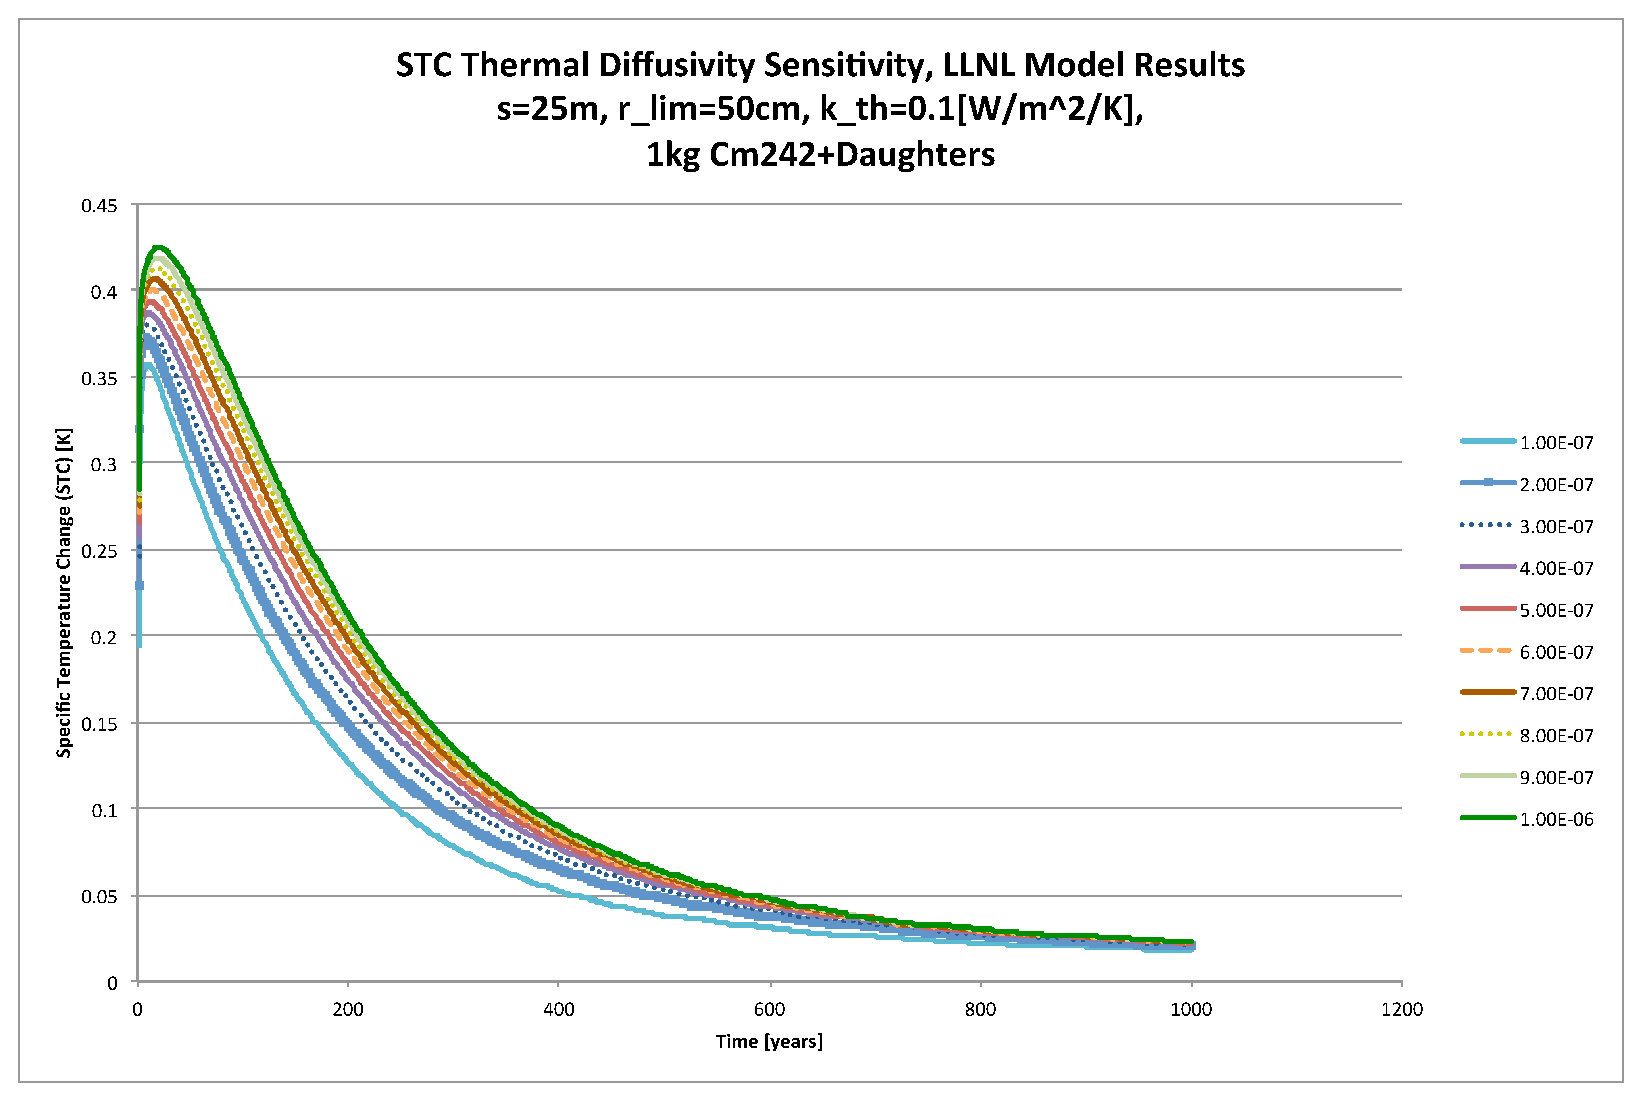
\includegraphics[height=0.7\textheight]{./thermal_demonstration/diffusivity/Cm242alpha_kth_low.eps}
\end{center}
\caption[$K_{th}$ Sensitivity to $\alpha_{th}$ for $k_{th}$]{Increased thermal diffusivity decreases thermal energy deposition 
(here represented by STC) in the near field (here $r_{calc} = 0.5m$).}
\label{fig:Cm242alpha_kth_low}
\end{figure}
}
\end{frame}


\begin{frame}[ctb!]
\frametitle{Cyder Thermal Diffusivity and Conductivity Sensitivity}
\footnotsize{
\begin{figure}[htbp!]
\begin{center}
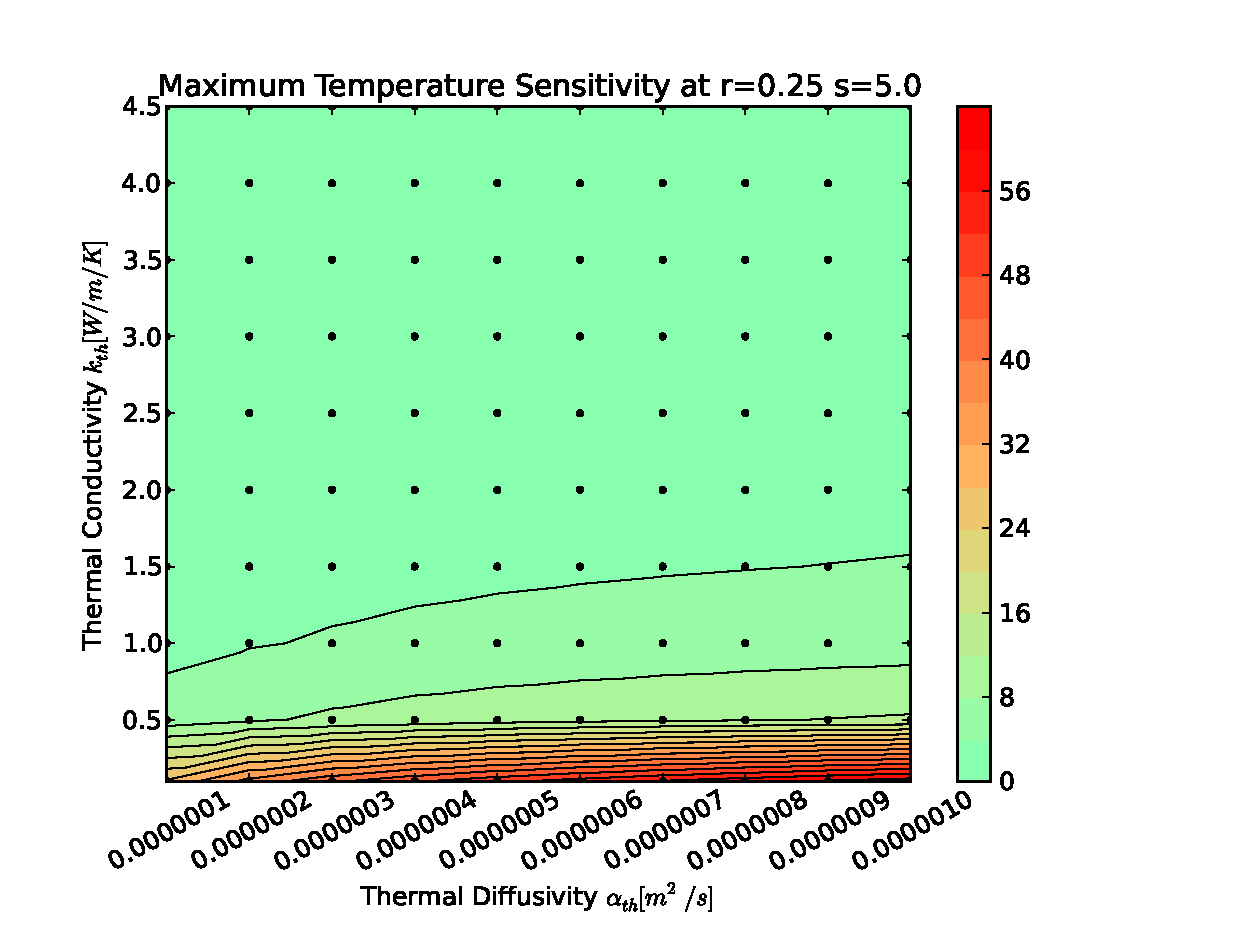
\includegraphics[height=0.7\textheight]{./thermal_demonstration/diffusivity/ak.eps}
\caption[$\alpha_{th}$ vs. $K_{th}$ Sensitivity in Cyder]{Cyder trends agree
with those of the LLNL model, in which increased thermal diffusivity results in 
decreased thermal depsoition in the near field. The above example thermal 
profile results from 10kg of $^{242}Cm$.} 
\label{fig:ar}
\end{center}
\end{figure}
}
\end{frame}

\begin{frame}[ctb!]
\frametitle{Cyder Thermal Diffusivity and Limiting Radius Sensitivity}
\footnotesize{
Further \Cyder analysis shows the importance of $K_{th}$ remains constant, but 
the importance of the limiting radius decreases with increasing $\alpha_{th}$.
\begin{figure}[htbp!]
\begin{center}
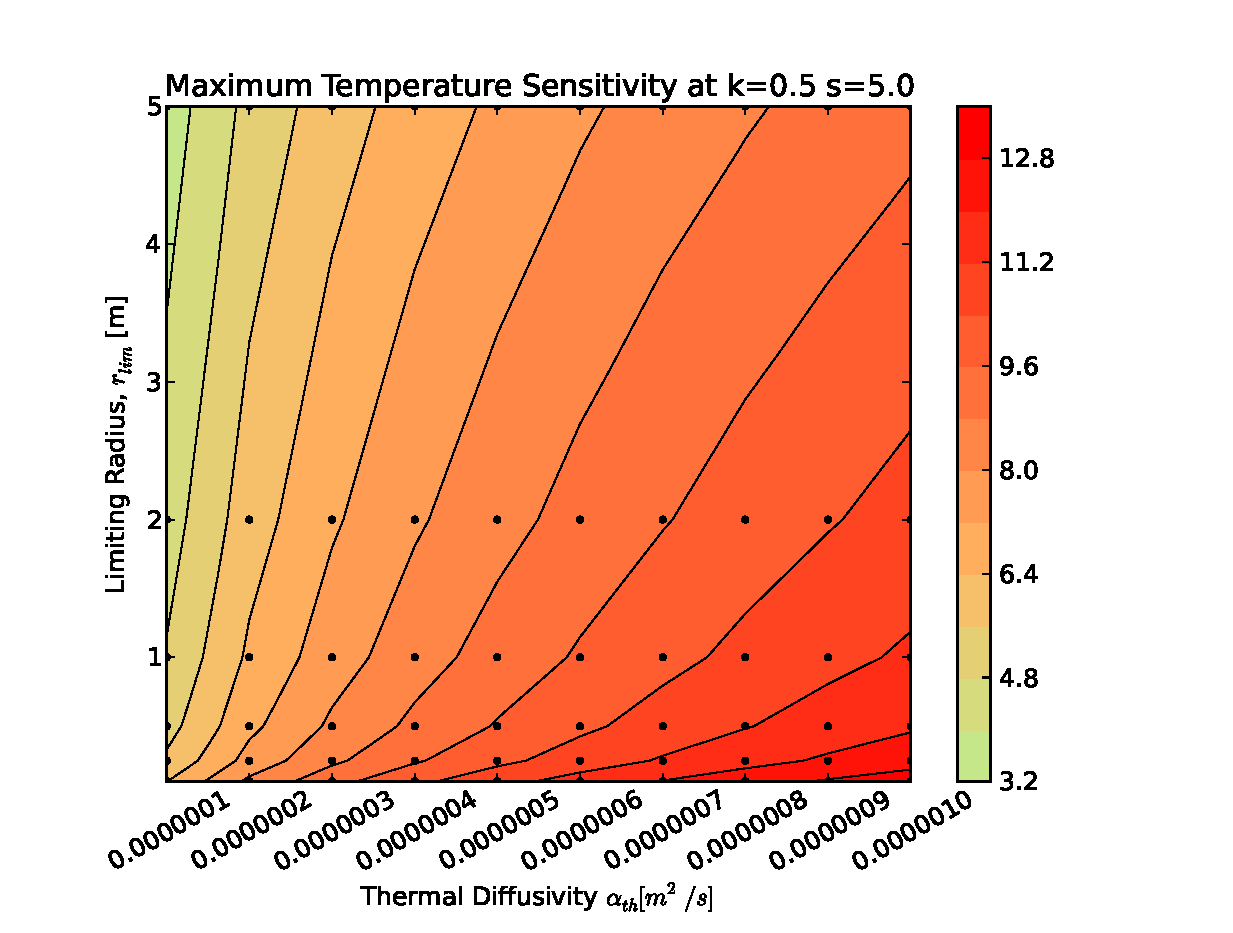
\includegraphics[height=0.7\textheight]{./thermal_demonstration/diffusivity/ar.eps}
\end{center}
\caption[$\alpha_{th}$ vs. $r_{lim}$ Sensitivity in Cyder]
{Cyder trends agree with 
those of the LLNL model. The importance of the limiting radius decreases with 
increased $K_{th}$. The above example thermal profile results from 10kg of 
$^{242}Cm$}
\label{fig:ak}
\end{figure}
}
\end{frame}
